\chapter{Синхронизација календара за \textit{оwnCloud} платформу}
\label{chap:ownCloudCalendarSynchronization}

У претходним поглављима описани су основни концепти технологија и окружења који су коришћени у развоју датог пројекта, са циљем да се читаоцу омогући да формира слику комплетног, заокруженог, решења. Сам пројекат, који је тема овог рада, може се посматрати као део тог решења. У овом поглављу фокус ће бити постављен на појашњења неких делова његове имплементације.

\section{Жељене функционалности}

Актуелна, званична, верзија \textit{оwnCloud} десктоп клијента обезбеђује само синхронизацију докумената који се налазе на \textit{оwnCloud} платформи. Основни циљ овог пројекта јесте да се развије решење, у виду мултиплатформског десктоп клијента, које би омогућило преузимање информација о креираним догађајима на \textit{оwnCloud} календару и приказ одговарајућих обавештења. Апликација има следећи скуп функционалности:
\begin{itemize}
	\item{\textit{синхронизација догађаја на захтев}},
	\item{\textit{аутоматска синхронизација догађаја}},
	\item{\textit{могућност управљања аутоматском синхронизацијом (потребна/није потребна, дефинисање временског интервала након којег ће се стартовати,...)}},
	\item{\textit{приступ делу за администрацију догађаја на веб порталу \textit{оwnCloud} платформе}},
	\item{\textit{приказ одговарајућег обавештења, непосредно пре почетка неког догађаја}},
	\item{\textit{преглед преузетих догађаја}}.
\end{itemize}

Ток активности које треба да обезбеде ове функционалности описан је на дијаграму \ref{fig:application_alogorithm}.

\begin{figure}[H]
	\centering
	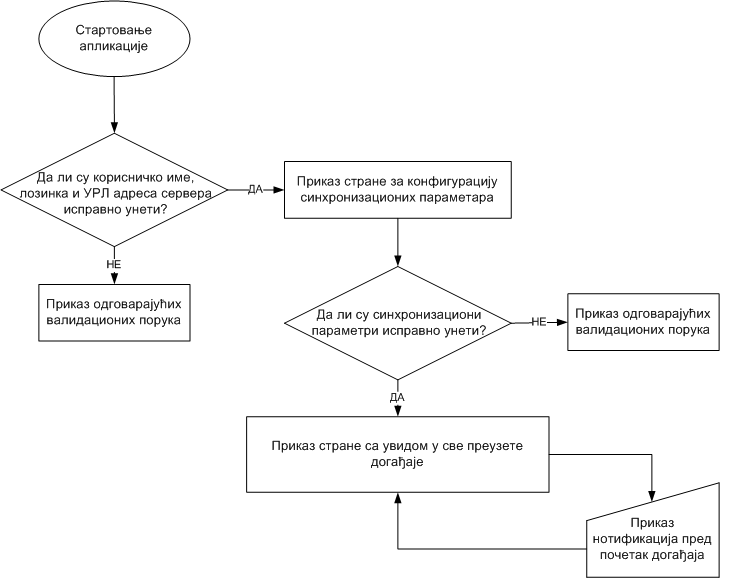
\includegraphics[scale=0.5]{slike/tok_aktivnosti.png}
	\caption{Дијаграм тока активности}
	\label{fig:application_alogorithm}
\end{figure}

На основу приказаног алгоритма  може се стећи јасна и потпуна слика о начину рада саме апликације. У наставку ће бити детаљније објашњене неке интересантније функционалности и биће приказани делови програмског кода, док се комплетан код пројекта може погледати на одговарајућем репозиторијуму\cite{svn_repo}.

\subsection{Аутентификација}

Аутентификација корисника на веб портал \textit{оwnCloud} платформе одрађена је коришћењем класа \textit{WebClient}, \textit{NetworkCredential} које су саставни део \textit{.NET Framework-a}.  Подаци унети на форми за пријаву на систем (Слика \ref{fig:login_form}), која се приказује након стартовања апликације, се прослеђују на верификацију:

\begin{figure}[H]
	\centering
	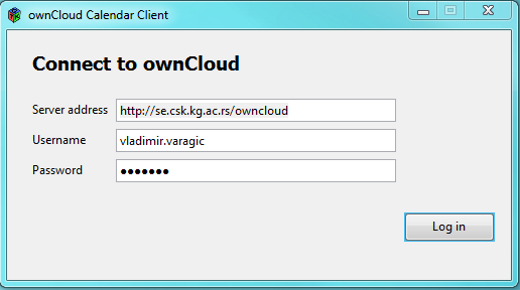
\includegraphics[scale=0.5]{slike/logInForm.png}
	\caption{Форма за пријаву на систем}
	\label{fig:login_form}
\end{figure}

Сви подаци на форми за пријаву су обавезни, па се у случају да неки податак није унет, прикаже одговарајући индикатор:

\begin{figure}[H]
	\centering
	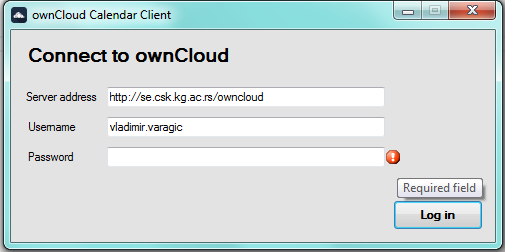
\includegraphics[scale=0.5]{slike/LogInFormReqiredFields.png}
	\caption{Форма за пријаву на систем}
	\label{fig:login_form_required}
\end{figure}

Такође, у случају да неки од података који се уносе приликом пријаве на апликацију (адреса сервера, корисничко име или лозинка) није исправан приказује се одговарајућа порука:

\begin{figure}[H]
	\centering
	\includegraphics[scale=0.5]{slike/logInFailed.png}
	\caption{Форма за пријаву на систем}
	\label{fig:login_form_failed}
\end{figure}

У супротном, ако су сви подаци исправни, корисник успешно приступа апликацији и приказује му се форма за синхронизацију догађаја са \textit{оwnCloud} календара.

\subsection{Синхронизација догађаја на захтев}

Као што је већ наведено у поглављу \textit{5.1.1 Аутентификација}, након успешног приступа апликацији кориснику се приказује форма за конфигурацију синхронизације:

\begin{figure}[H]
	\centering
	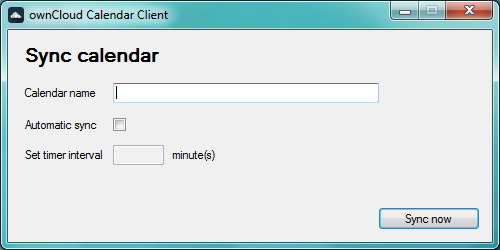
\includegraphics[scale=0.5]{slike/SyncCalendar.png}
	\caption{Синхронизација догађаја са \textit{оwnCloud} календара}
	\label{fig:sync_calendar}
\end{figure}


\textit{OwnCloud} платформа омогућава кориснику да на порталу води више различитих календара тј. да календар дели у различите категорије. 

\begin{figure}[H]
	\centering
	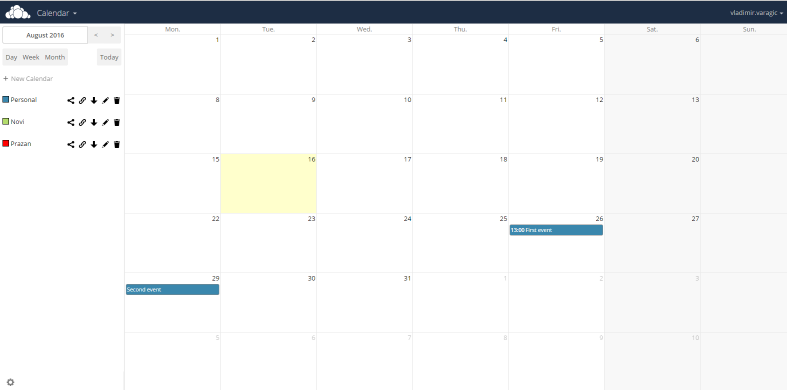
\includegraphics[scale=0.5]{slike/ownCloudCalendar.png}
	\caption{\textit{OwnCloud} календар}
	\label{fig:own_cloud_calendar}
\end{figure}

Са друге стране, синхронизацијом се у једном тренутку могу преузети само догађаји који су везани за једну категорију, тако да је назив календара обавезан податак приликом синхронизације.